\section{La función de relación humana}

Como el resto de los vertebrados, las personas tenemos una función de relación muy desarrollada (Figura \ref{fig:relacion}), que consta de tres procesos: recepción de estímulos, procesamiento de la información y ejecución de las respuestas.

\vspace{3mm}
\textbf{La recepción de estímulos}

\vspace{3mm}
La llevan a cabo los \textbf{órganos receptores}, también conocidos como \textbf{órganos de los sentidos}. Estos órganos detectan luz, vibraciones sonoras, sustancias, temperatura o contactos, y transforman estos estímulos en señales llamadas \textbf{impulsos nerviosos}.

\vspace{3mm}
\textbf{El procesamiento de la información}

\vspace{3mm}
Lo lleva a cabo el \textbf{sistema nervioso}, que es una compleja red de células llamadas \textbf{neuronas}, especializadas en transmitir los impulsos nerviosos por todo el cuerpo. El sistema nervioso recoge los impulsos nerviosos de los órganos receptores y los lleva hasta \textbf{centros de coordinación}. Allí, esos impulsos se interpretan y se convierten en impulsos nerviosos de respuesta. Dichos impulsos se envían a los órganos que ejecutan dichas respuestas.

\vspace{3mm}
\textbf{La ejecución de las respuestas}

\vspace{3mm}
La llevan a cabo los órganos efectores, que realizan acciones cuando reciben los impulsos nerviosos. Los principales son:

\begin{itemize}
    \item Los \textbf{músculos}, tanto la musculatura esquelética como el corazón o los músculos del tubo digestivo, que son capaces de producir movimientos.
    \item Las \textbf{glándulas}, que producen diversas sustancias químicas como la saliva o las hormonas, que tienen, a su vez, efectos en otros órganos.
\end{itemize}

\begin{figure}[!ht]
    \centering
    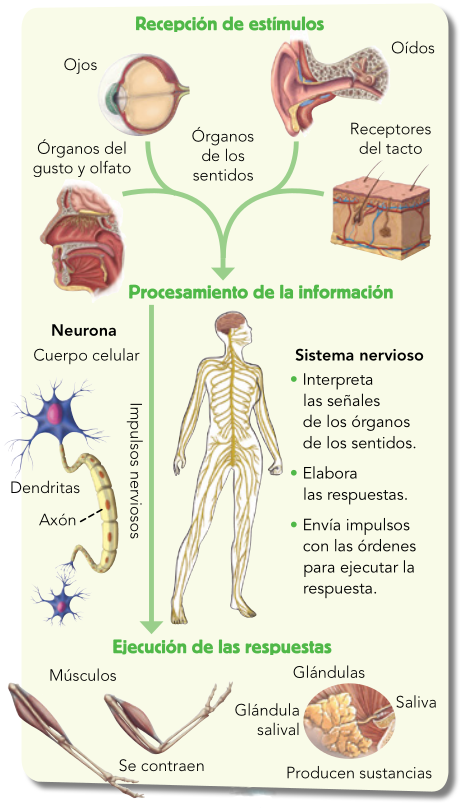
\includegraphics[width=0.4\linewidth]{Tema3/11_Relacion.png}
    \caption{La función de relación humana}
    \label{fig:relacion}
\end{figure}

\subsection{Los órganos receptores}

\subsubsection{Esquema básico de un órgano receptor}

Todos los órganos receptores (Figura \ref{fig:organos-receptores}) tienen un esquema básico común:

\begin{itemize}
    \item Una parte destinada a recibir el estímulo y muy especializada para captar un estímulo en particular.
    \item Unas células receptoras, que se encargan de transformar los estímulos en señales nerviosas.
    \item Unos nervios sensoriales, que envían esas señales al sistema nervioso para que las interprete.
\end{itemize}

\begin{figure}[!ht]
    \centering
    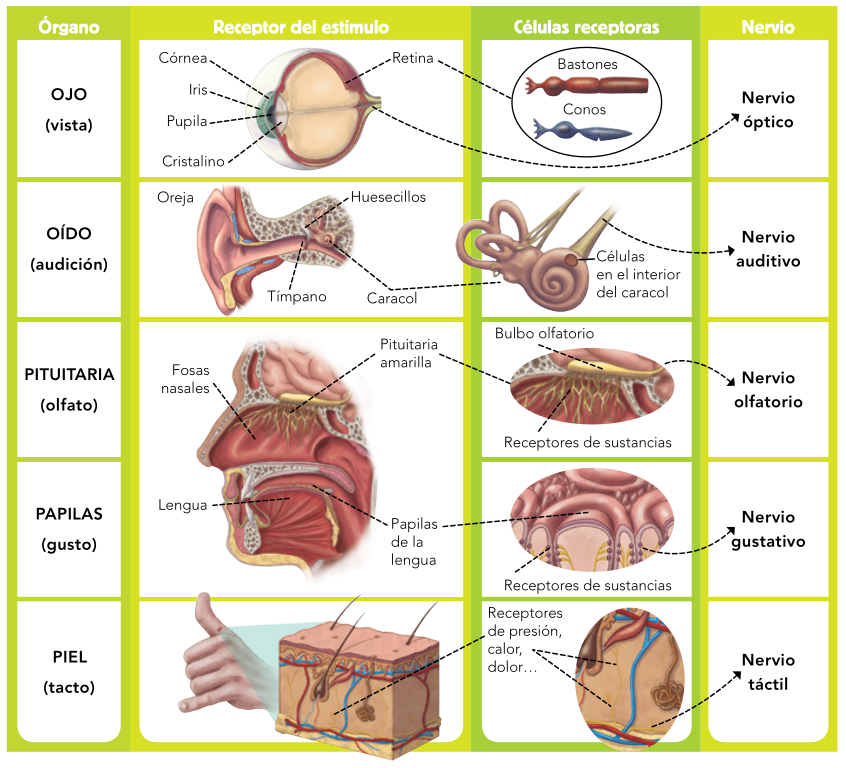
\includegraphics[width=0.6\linewidth]{Tema3/12_Organos_receptores.png}
    \caption{Esquema básico de los órganos receptores}
    \label{fig:organos-receptores}
\end{figure}

\subsection{El sistema nervioso}

El sistema nervioso (Figura \ref{fig:sistema-nervioso}) se organiza en dos partes: el sistema nervioso central y el sistema nervioso periférico.

\begin{figure}[!ht]
    \centering
    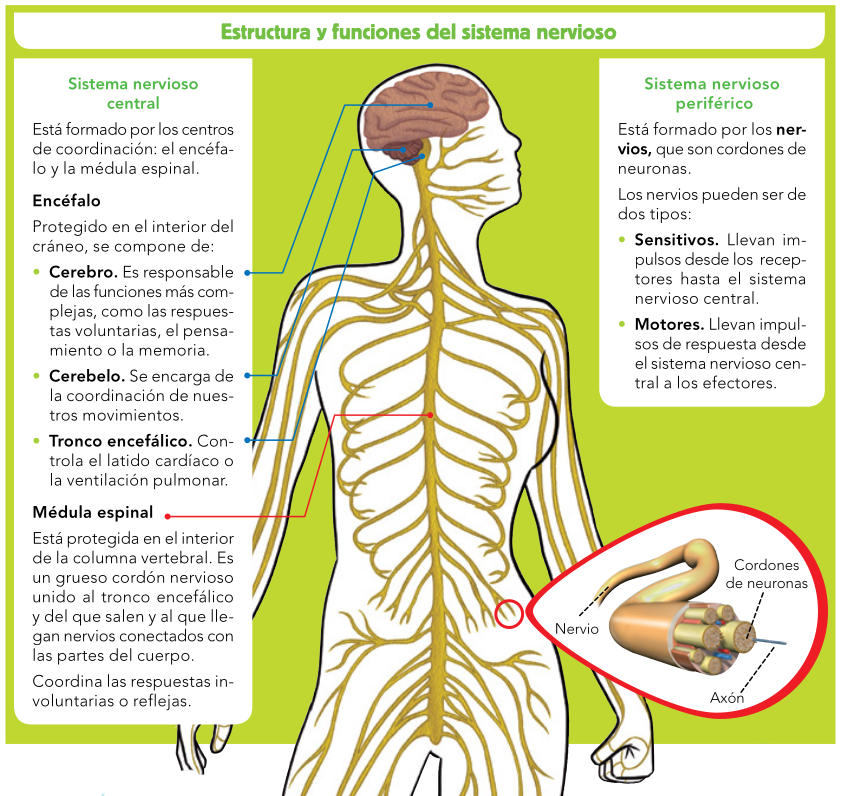
\includegraphics[width=0.6\linewidth]{Tema3/13_Estructura_funciones_sistema_nervioso.png}
    \caption{Estructura y funciones del sistema nervioso}
    \label{fig:sistema-nervioso}
\end{figure}

\subsubsection{Los órganos efectores}

Los órganos efectores son aquellos que realizan una acción cuando les llega una orden de respuesta a través del sistema nervioso. Los principales son los músculos y las glándulas.

\subsubsection{Los músculos}

Los músculos son órganos formados por células capaces de contraerse al recibir un impulso nervioso. De este modo, producen los movimientos del cuerpo.

\vspace{3mm}
Los seres humanos tenemos en nuestro cuerpo dos tipos de músculos:

\begin{itemize}
    \item \textbf{Músculos esqueléticos}. Como indica su nombre, funcionan en combinación con el esqueleto, están unidos a los huesos mediante tendones, y juntos constituyen el aparato locomotor. 
    \item \textbf{Músculos no esqueléticos}. Son músculos no relacionados con el esqueleto. Producen el movimiento de órganos como el corazón, el iris del ojo y el tubo digestivo.
\end{itemize}

\begin{figure}[!ht]
    \centering
    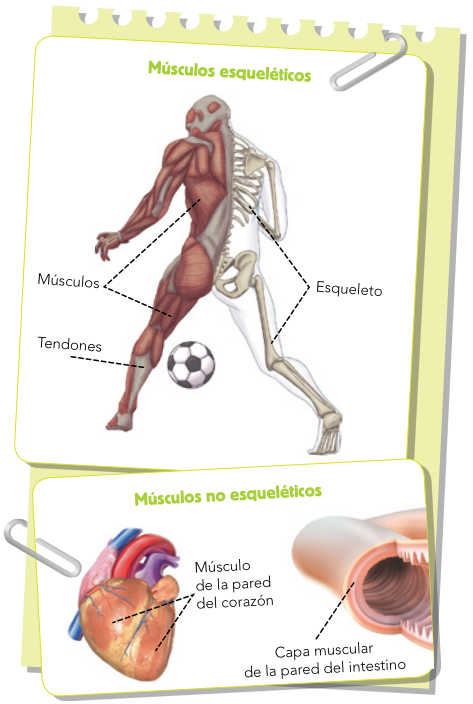
\includegraphics[width=0.5\linewidth]{Tema3/14_Musculos.png}
    \caption{Tipos de músculos}
    \label{fig:musculos}
\end{figure}

\subsubsection{Las glándulas}

Las glándulas son órganos que, cuando reciben una señal del sistema nervioso, producen determinadas sustancias como saliva, sudor, jugos digestivos, hormonas...

\subsection{Relación y salud}

El ambiente y ciertos malos hábitos pueden perjudicar a los órganos de los sentidos, al sistema nervioso o a los efectores, y alterar nuestra función de relación. Para prevenir algunos daños, además de ir a revisiones médicas periódicas, se pueden tomar ciertas medidas.

\subsubsection{El cuidado de los órganos de los sentidos}

Algunos hábitos saludables pueden prevenir enfermedades de los órganos de los sentidos:

\begin{itemize}
    \item \textbf{Cuidar la vista}. Conviene utilizar gafas de sol en la playa o la nieve, leer con suficiente luz, no pasar mucho tiempo mirando pantallas electrónicas, tomar alimentos con vitaminas, como frutas o verduras...
    \item \textbf{Cuidar los oídos}. Se debería evitar exponerse a ruidos fuertes o prolongados, introducir objetos en los oídos ni para secarlos, abusar de los auriculares...
    \item \textbf{Cuidar el olfato y el gusto}. Para ello, hay que mantener limpias tu boca y tus fosas nasales.
    \item \textbf{Cuidar el sentido del tacto}. Se consigue con una adecuada higiene de la piel y utilizando protección solar.
\end{itemize}

\subsubsection{El cuidado del sistema nervioso}

Debemos cuidar nuestro sistema nervioso tanto en el aspecto físico como en el emocional.

\vspace{3mm}
\textbf{El cuidado físico del sistema nervioso}

\begin{itemize}
    \item \textbf{Conviene protegerse de golpes} en la cabeza o la espalda, ya que el encéfalo o la columna podrían dañarse.
    \item \textbf{Hay que evitar siempre las bebidas alcohólicas, el tabaco y otras drogas}. Estas sustancias llegan al cerebro y pueden ocasionar daños en este órgano, especialmente en las personas jóvenes, como vosotras y vosotros, que estáis en pleno desarrollo.
\end{itemize}

\textbf{La salud emocional}

\vspace{3mm}
Para conseguir una buena salud emocional, es importante relacionarse con otras personas, \textbf{cuidar la autoestima, mostrar empatía,} adoptar una \textbf{actitud positiva}, intentar \textbf{superar las dificultades}...

\vspace{3mm}
\textbf{El cuidado de los efectores}

\vspace{3mm}
Para mantener en buen estado nuestro aparato locomotor, conviene seguir estos hábitos:

\begin{itemize}
    \item \textbf{Hacer ejercicio de forma regular} y adecuada para tu edad y tu fuerza. Asimismo, conviene realizar un calentamiento antes de empezar la actividad y unos estiramientos al finalizarla.
    \item \textbf{Mantener unas posturas que no dañen los músculos, la columna vertebral o las articulaciones} al caminar, al sentarse durante un tiempo, al cargar algo de peso...
    \item \textbf{Evitar las actividades con un exceso de peligro y utilizar protecciones adecuadas} al montar en bici, patinar, ir en coche...
\end{itemize}